\documentclass{article}
\usepackage[margin=1in]{geometry}
\usepackage{amsmath,amsthm,amssymb}
\usepackage{bbm,enumerate,mathtools}
\usepackage{tikz,pgfplots}
\usepackage{chessboard}
\usepackage[hidelinks]{hyperref}
\usepackage{multicol} % Problem 35
\usepackage{xstring} % Difficulty command
\usetikzlibrary{shapes.geometric}

\newenvironment{question}{\begin{trivlist}\item[\textbf{Question.}]}{\end{trivlist}}
\newenvironment{note}{\begin{trivlist}\item[\textbf{Note.}]}{\end{trivlist}}
\newenvironment{references}{\begin{trivlist}\item[\textbf{References.}]}{\end{trivlist}}
\newenvironment{related}{\begin{trivlist}\item[\textbf{Related.}]\end{trivlist}\begin{enumerate}}{\end{enumerate}}

\newcommand\score[1]{
\pgfmathsetmacro\pgfxa{#1+1}
\tikzstyle{scorestars}=[
  star,
  star points=5,
  star point ratio=2.25,
  draw,
  inner sep=3pt,
  anchor=outer point 5
]
  \begin{tikzpicture}[baseline]
    \draw[opacity=0] (0,-0.5) rectangle (0,0.2); % Workaround for whitespace at the bottom.
    \foreach \i in {1,...,4} {
      \pgfmathparse{(\i<=#1?"yellow":"gray")}
      \edef\starcolor{\pgfmathresult}
      \draw (\i*4.5ex,0) node[name=star\i,scorestars,fill=\starcolor]  {};
    }
  \end{tikzpicture}
}

\newcommand{\difficulty}[1]{%
  \IfEqCase{#1}{%
      {1}{
        
\begin{tikzpicture}[scale=0.7, baseline=0.9mm]%
          \definecolor{slopegreen}{rgb}{0.0, 0.5, 0.0}%
          \fill[slopegreen] (0.5,0.5) circle (0.5);%
        \end{tikzpicture}%
      }%
      {2}{
        
\begin{tikzpicture}[scale=0.7, baseline=0.9mm]%
          \definecolor{slopeblue}{rgb}{0.0, 0.44, 1.00}
          \fill[slopeblue] (0,0) rectangle (1,1);%
        \end{tikzpicture}%
      }%
      {3}{
\begin{tikzpicture}[scale=0.7, baseline=0.9mm]\fill (0,0.5)--(0.5, 0)--(1,0.5)--(0.5,1)--cycle; \end{tikzpicture}}%
      {4}{
\begin{tikzpicture}[scale=0.7, baseline=0.9mm]\fill (0.25,0)--(0,0.5)--(0.25,1)--(0.5,0.5)--cycle; \fill (0.75,0)--(0.5,0.5)--(0.75,1)--(1,0.5)--cycle;\end{tikzpicture}}%
      % you can add more cases here as desired
  }[\PackageError{difficulty}{Undefined difficulty level: #1}{}]%
}%
\newcommand{\rating}[2]{\difficulty{#1}\\\score{#2}\\}


\begin{document}
\rating{1}{3}
  Consider a $n \times m$ grid of ones and zeroes, which represent the heights of the
  cells. It rains, and the grid fills up with the rain moving horizontally and
  vertically.
\begin{figure}[ht!]
  \centering
  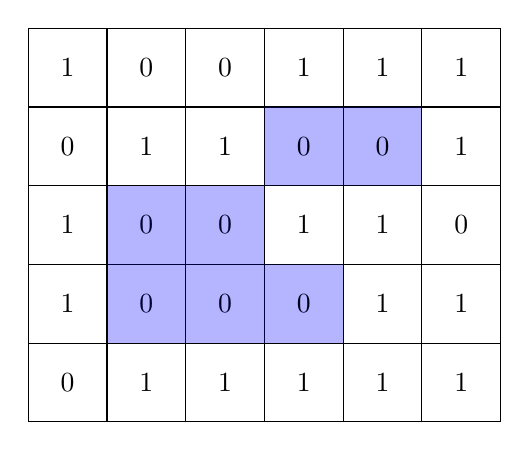
\begin{tikzpicture}
    \draw (0,0) grid (6,5);
    \foreach \x/\y/\n in {
      0/0/0, 0/1/1, 0/2/1, 0/3/0, 0/4/1,
      1/0/1, 1/1/0, 1/2/0, 1/3/1, 1/4/0,
      2/0/1, 2/1/0, 2/2/0, 2/3/1, 2/4/0,
      3/0/1, 3/1/0, 3/2/1, 3/3/0, 3/4/1,
      4/0/1, 4/1/1, 4/2/1, 4/3/0, 4/4/1,
      5/0/1, 5/1/1, 5/2/0, 5/3/1, 5/4/1
    } {
      \node at (0.5 + \x, \y + 0.5) {\n};
      \fill[blue, fill opacity=0.01]
        (1,1) rectangle (4,2)
        (1,2) rectangle (3,3)
        (3,3) rectangle (5,4)
      ;
    }
  \end{tikzpicture}
  \caption{
    An example of five non-parallel centered squares in the size 6 square, and
    an example of three non-parallel non-centered squares that do not share any
    lattice points.
  }
\end{figure}

\begin{question}
  What is the expected area of a lake? Of the sum of all lakes?
\end{question}

\begin{related}
  \item What is the expected number of lakes? Of islands? Of lakes on islands?
  \item What if water can flow diagonally too?
  \item What if the heights can take on arbitrary values?
  \item What if there is a border around the grid of height $k$?
  \item What if the cell is height $0$ with probability $p$ and height $1$ with probability $(1-p)$?
  \item How does this generalize to triangular/hexagonal grids? More dimensions?
  \item How does this generalize to a cylinder?
\end{related}

\begin{references}
  \item Problem 86.
  \item \url{https://codegolf.stackexchange.com/q/2638/53884}
\end{references}

\end{document}
